\documentclass{article}

\usepackage[nonatbib,final]{neurips_2020}

\usepackage[utf8]{inputenc} % allow utf-8 input
\usepackage[T1]{fontenc}    % use 8-bit T1 fonts
\usepackage{hyperref}       % hyperlinks
\usepackage{url}            % simple URL typesetting
\usepackage{booktabs}       % professional-quality tables
\usepackage{amsfonts}       % blackboard math symbols
\usepackage{nicefrac}       % compact symbols for 1/2, etc.
\usepackage{microtype}      % microtypography
\usepackage{graphicx}
\usepackage{placeins}       % for \FloatBarrier
\usepackage{floatflt}
\usepackage{subcaption}     % for subfigure
\usepackage[backend=biber,style=ieee,sorting=none]{biblatex}
\addbibresource{report.bib}

\title{Identification of microglia in mouse brain tissue using a convolutional 
neural network \\
\large SENG 474: Data Mining, University of Victoria \\
}

\author{
    Scott Howard
    \And
    Elliot Lupini
    \And
    Leo McKee-Reid
}
\date{April 19, 2022}

\begin{document}

\maketitle

\section{Introduction}

In order to better understand the brain and cure neurodegenerative diseases, 
neuroscientists image the brain to study its structure on a macro, cellular, 
and molecular scale. A common practice in cellular neuroscience is to use 
powerful microscopes to image very thinly sliced animal brain tissues that 
have been stained so that a specific cell stands out. As imaging technology 
improves, the amount of image data that needs to be manually analyzed has 
become a major bottleneck. In this project, we aim to replace the tedious 
process of manual cell identification with an automated process using a 
convolutional neural network (CNN) to detect microglia (a type of brain cell) 
in light microscopy images of mouse brain tissue. The image data we have used 
to train and test our model (see Figure \ref{fig:hippocampus}) has been 
provided by the Tremblay Lab --- a neuroscience lab at the University of 
Victoria with a research focus on microglia and how it impacts learning, 
stress, disease, and aging in the brain \parencite{tremblay}.

\begin{figure}[ht]
  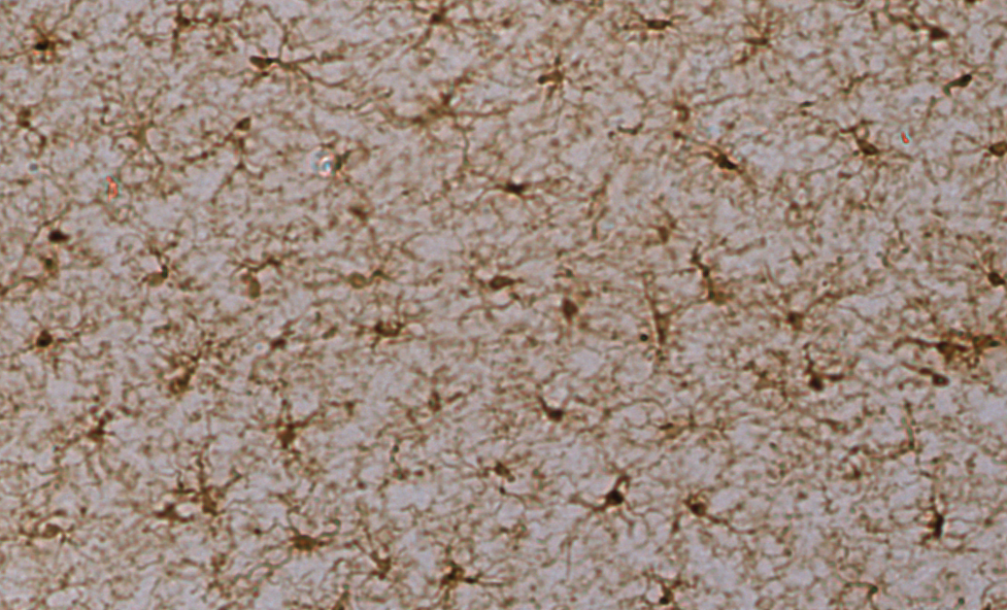
\includegraphics[width=0.7\textwidth]{hippocampus.png}
  \centering
  \captionsetup{width=0.7\textwidth}
  \caption{A slice of mouse brain tissue, imaged with light microscopy at the 
  Tremblay Lab. Most of the dark spots in the image are microglia cells --- the 
  target of this experiment.}
  \label{fig:hippocampus}
\end{figure}

\section{The Problem}

The Tremblay Lab is currently researching how the density and distribution of 
microglia change in a mouse hippocampus. Researchers are required to manually 
label every microglia in tons of images, which both takes a lot of time and 
is sensitive to human error. To remove this research bottleneck, we have 
built a CNN to automate identifying microglia. The model was trained on 
datasets adapted from images that had been previously annotated manually by 
the Tremblay Lab (see Figure \ref{fig:classification-dot}). Therefore, the 
input to our model is a raw, light microscopy image of a mouse hippocampus, 
and the output is the segmentation of the cell body. Researchers in the Lab 
can send this segmentation layer generated by the CNN into an image 
processing tool called ImageJ, which outputs the properly formatted density 
and distribution results they need.

\begin{figure}[ht]
  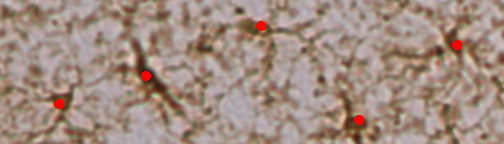
\includegraphics[width=0.7\textwidth]{classification-dot.png}
  \centering
  \captionsetup{width=0.7\textwidth}
  \caption{A cropped input image with manually labeled red dots to indicate where 
  the center of each microglia is.}
  \label{fig:classification-dot}
\end{figure}

As shown in Figures \ref{fig:hippocampus} and \ref{fig:classification-dot}, 
microglia are very irregularly shaped, and some cell arms can bend in such a 
way that it looks like there is another cell body. This makes their 
identification quite challenging, but at least this is a challenge for both a 
CNN and a human annotator, and a CNN is typically easier and quicker to 
re-train.

The Tremblay Lab also wishes to build a similar CNN tool to do automatic 
morphology analysis. This is a much more challenging problem, as instead of 
simply identifying the center of each cell, it needs to trace around the cell 
body (i.e., segmentation) to determine the size and shape. The construction 
of this additional CNN is outside the scope of our project; however, since 
the model's structure will be very similar to our cell identification CNN, we 
have built a testing metric for this morphology CNN. The work we have done in 
this project will therefore be the foundation for the morphology CNN, which 
will be trained and tested this summer on a more detailed dataset. 

The formal goal of this project is therefore to train and test a CNN for 
microglia identification, and to develop the testing metric for the future 
morphology CNN. 

\section{Background}

Object detection problems similar to this are common within computer vision 
(e.g., detecting a vehicle, a person, tumors, broken bones, etc.). The last 
decade has seen a large increase in neuroscience labs applying CNNs of this 
kind to cell detection and segmentation. There are also a few free, 
plug-and-play software programs that do segmentation — such as 
Ilastik \parencite{ilastik}. However, since the CNN models developed in other 
labs are fine-tuned to their datasets (and the fact that most labs are 
competing for funding and don't want to share their custom built tools), most 
neuroscience labs have to build their own CNNs. In addition, programs like 
Ilastik don't yield a high enough testing accuracy unless the objects that 
are being classified really stand out from any other object in the image. For 
these reasons, the Tremblay Lab has decided to begin building their own CNN 
models, with our project being their first.

A CNN is a type of fully connected neural network that is commonly used for 
image classification. In order to recognize specific objects, a CNN 
simplifies an input image by applying \textit{convolutions} (a type of filter)
to create feature maps, which are then run through an activation function, 
and finally that output grid of pixels are pooled before sending the 
resulting pixel values into a neural network. Before training, these 
convolutions (which are just a NxN grid of zeros or ones) are randomly 
generated. However, through backpropagation, the convolutions begin to change 
in order to minimize the error of the network's prediction. This results in a 
set of convolutions that are finely tuned to produce the best predictions 
based on the training data. 

Due to the way a CNN filters the input image, the best way to identify the 
center of microglia is to simply segment the cell body (since CNNs are good 
at finding the boundary of objects). This is the reason why our density and 
distribution CNN will be very similar to the post-project morphology CNN: 
they both have to trace out the cell body.

While segmentation software like Ilastik are not yet accurate enough for the 
data we've been provided, there are python libraries --- such as 
Gunpowder \parencite{gunpowder} and PyTorch \parencite{pytorch} --- that make 
the development of this type of model much easier. In the early stages of the 
project, we were able to use the model parameters from a tutorial provided by 
Gunpowder \parencite{gunpowder-tutorial} that we were able to adapt in order 
to generate prediction images that qualitatively looked very accurate.

This type of analysis is incredibly valuable, as it will increase our 
collective understanding of how microglia can contribute to, and fight against,
neurodegeneration. There are a number of projects in the lab that are already 
waiting to use our classification tool.

\begin{figure}[ht]
  \begin{subfigure}{0.49\textwidth}
    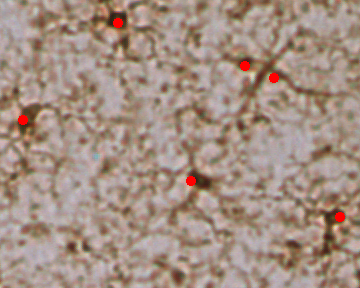
\includegraphics[width=0.7\textwidth]{classification2-dots.png}
    \centering
    \caption{}
    \label{fig:classification2-dots}
  \end{subfigure}
  \begin{subfigure}{0.49\textwidth}
    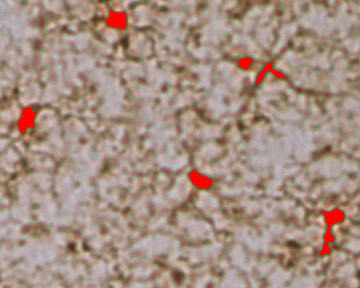
\includegraphics[width=0.7\textwidth]{classification2-cell.png}
    \centering
    \caption{}
    \label{fig:classification2-cell}
  \end{subfigure}
  \captionsetup{width=0.85\textwidth}
  \caption{From the provided segmentation using dots (a), we produced a cell
  segmentation layer (b) to use in training the model.}
\end{figure}

\section{Method}

The approach we took can be broken down into 4 steps: preprocessing, training,
prediction, and post-processing. The microglia in the images that were given 
to us by the Tremblay Lab were labeled with a single dot in the middle of the 
cell body (see Figure \ref{fig:classification2-dots}). After training and 
testing our initial model on these single dot labels, it was clear that our 
CNN would train much better if the whole cell body was labeled (see Figure
\ref{fig:classification2-cell}). Using the image editing tool GIMP, we were 
able to transform the original single dots to cover the entire cell body by 
thresholding the image, then only keeping the dark patches that touched the 
single dots. Now that we had the correct labels, we used Gunpowder to 
streamline the training/testing pipeline. This python library not only 
provides a clean pipeline, but is also advantageous for computer vision tasks.
It allows for easy image manipulation as well as integrating with PyTorch. We 
wanted to get the most out of our labeled training data, so we used Gunpowder 
to randomly sample the larger training images into smaller sizes, then 
performed linear transforms on them to generate even more images. This 
increased our number of training images by a factor of ten. The current 
parameters of our model are based on a Gunpowder tutorial, which implements a 
U-Net \parencite{unet} through a library interface to PyTorch. The 
predictions made by the model are passed through a post-processing routine to 
eliminate low pixel activations that correspond to ``unconfident'' predictions 
(see Figure \ref{fig:masked-pixels}). 

\begin{figure}[ht]
  \begin{subfigure}{0.25\textwidth}
    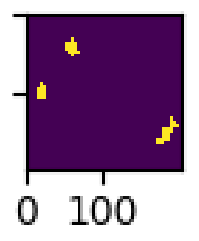
\includegraphics[width=0.6\textwidth]{pixel-mask-seg.png}
    \centering
    \caption{Expected}
  \end{subfigure}%
  \begin{subfigure}{0.25\textwidth}
    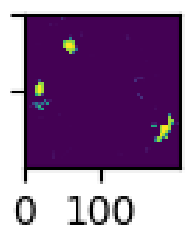
\includegraphics[width=0.6\textwidth]{pixel-mask-pred.png}
    \centering
    \caption{Model prediction}
  \end{subfigure}%
  \begin{subfigure}{0.25\textwidth}
    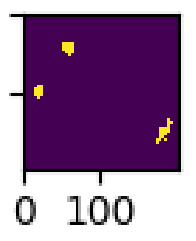
\includegraphics[width=0.6\textwidth]{pixel-mask-masked.png}
    \centering
    \caption{Masked prediction}
  \end{subfigure}
  \centering
  \captionsetup{width=0.7\textwidth}
  \caption{A pixel mask was applied (c) to the model's prediction (b),
  resulting in a better prediction of the expected (a).}
  \label{fig:masked-pixels}
\end{figure}

To evaluate the efficacy of the model, we developed the following metrics to 
quantitatively score the model’s predictions:
\begin{enumerate}
\item \textbf{Naive Count Difference}: Count the number of microglia cells 
(identified as clusters) in the expected layer and the predicted layer, and 
return the absolute value of the difference in counts. Cell locations are not 
considered in this metric, so the reported error will not capture incorrectly 
located predictions.
\item \textbf{Pixel Difference}: Perform a pixel-wise XOR between the 
expected and predicted layers and return the number of pixels that remain 
activated. Pixels that remain activated are the pixels that the model 
incorrectly predicted.
\item \textbf{Count Difference}: An improved version of the naive count 
difference metric, this metric takes into account the location of each 
predicted cell cluster. A predicted cluster is considered the same as the 
expected cluster if their centroids are within a tolerance of each other (5 
pixels). The improved count difference returns the sum of the false positives 
and false negatives.
\end{enumerate}

With the development of the improved count difference metric, it was 
determined that the naive count difference was no longer necessary, and has 
not been included in any of the data visualizations. For both the pixel 
difference and count difference metrics, it was important to normalize the 
data so that an appropriate comparison could be made between the smaller 
training samples and the larger test samples. To that end, the count 
difference metric was normalized by the number of expected clusters, and the 
pixel difference metric was normalized by the number of pixels in the image 
and represented as a percentage.

\section{Results}

The benefit of a computer vision task is that we can qualitatively gauge how 
the model is performing, although quantitative measures are absolutely 
necessary to properly improve the predictions. Figures 
\ref{fig:training-sample} and \ref{fig:test-sample} illustrate the output 
from the model alongside the raw image and ground truth. It's important to 
see the output in order to properly understand the quantitative measures.

\begin{figure}[ht]
  \begin{subfigure}{0.2\textwidth}
    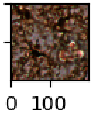
\includegraphics[width=0.7\textwidth]{training-sample-raw.png}
    \centering
    \caption{Raw}
  \end{subfigure}%
  \begin{subfigure}{0.2\textwidth}
    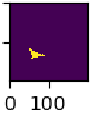
\includegraphics[width=0.7\textwidth]{training-sample-seg.png}
    \centering
    \caption{Expected}
  \end{subfigure}%
  \begin{subfigure}{0.2\textwidth}
    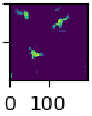
\includegraphics[width=0.7\textwidth]{training-sample-pred.png}
    \centering
    \caption{Model prediction}
  \end{subfigure}%
  \begin{subfigure}{0.2\textwidth}
    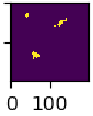
\includegraphics[width=0.7\textwidth]{training-sample-masked.png}
    \centering
    \caption{Masked prediction}
  \end{subfigure}
  \centering
  \captionsetup{width=0.9\textwidth}
  \caption{A sample training output, showing the raw input image, the ground 
  truth, the raw output of the model, and the masked output.}
  \label{fig:training-sample}
\end{figure}

\begin{figure}[ht]
  \centering
  \begin{subfigure}{0.24\textwidth}
    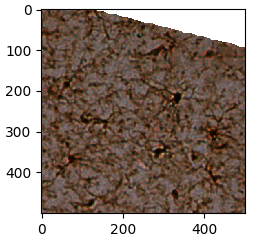
\includegraphics[width=0.9\textwidth]{test-sample-raw.png}
    \centering
    \caption{Raw}
  \end{subfigure}%
  \begin{subfigure}{0.24\textwidth}
    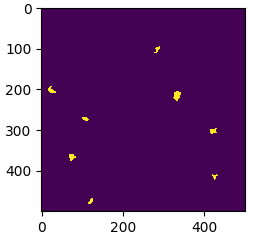
\includegraphics[width=0.9\textwidth]{test-sample-seg.png}
    \centering
    \caption{Expected}
  \end{subfigure}%
  \begin{subfigure}{0.24\textwidth}
    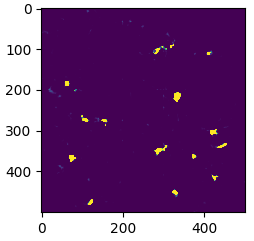
\includegraphics[width=0.9\textwidth]{test-sample-pred.png}
    \centering
    \caption{Model prediction}
  \end{subfigure}%
  \begin{subfigure}{0.24\textwidth}
    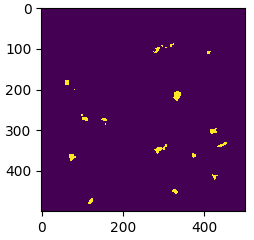
\includegraphics[width=0.9\textwidth]{test-sample-masked.png}
    \centering
    \caption{Masked prediction}
  \end{subfigure}
  \captionsetup{width=0.9\textwidth}
  \caption{A sample test output, showing the raw input image, the ground truth,
  the raw output of the model, and the masked output.}
  \label{fig:test-sample}
\end{figure}

The results (see Table \ref{tbl:epoch-summary} and Figure 
\ref{fig:epoch-summary}) summarize the performance of the count difference 
and pixel difference metrics over all epochs. Each training epoch consisted 
of 720 images and then was tested on 19 images (larger size, but same 
resolution to not affect model performance). The count difference metric was 
normalized by the number of actual/expected clusters in the image so the 
training and testing scores can be compared. The pixel difference metric was 
normalized by the size of the input image, which was 200x200 for the training 
dataset, and 500x500 for the test dataset. The resulting value was the number 
of differing pixels, represented as a percentage.

\begin{table}[ht]
  \captionsetup{width=\textwidth}
  \caption{Aggregated data from each epoch of the model. Each epoch consists 
  of one round of training the model, followed by validation with the test set.}
  \label{tbl:epoch-summary}
  \centering
  \begin{subtable}{0.5\textwidth}
    \caption{Training data}
    \begin{tabular}{crrr}
      \toprule
      Epoch & \shortstack{Count \\ difference} & \shortstack{Pixel \\ difference (\%)} \\
      \midrule
        01  &             0.60 &             0.20 \\
        02  &             0.48 &             0.18 \\
        03  &             0.46 &             0.18 \\
        04  &             0.63 &             0.18 \\
        05  &             0.55 &             0.18 \\
        06  &             0.49 &             0.17 \\
        07  &             0.73 &             0.18 \\
        08  &             0.58 &             0.16 \\
        09  &             0.50 &             0.17 \\
        10  &             0.60 &             0.17 \\
        11  &             0.66 &             0.17 \\
        12  &             0.68 &             0.18 \\
      \bottomrule
    \end{tabular}
  \end{subtable}%
  \begin{subtable}{0.5\textwidth}
    \caption{Test data}
    \begin{tabular}{crrr}
      \toprule
      Epoch & \shortstack{Count \\ difference} & \shortstack{Pixel \\ difference (\%)} \\
      \midrule
        01  &             1.16 &             0.18 \\
        02  &             0.93 &             0.16 \\
        03  &             1.19 &             0.19 \\
        04  &             0.93 &             0.15 \\
        05  &             1.93 &             0.17 \\
        06  &             1.32 &             0.16 \\
        07  &             0.99 &             0.17 \\
        08  &             0.94 &             0.15 \\
        09  &             1.75 &             0.18 \\
        10  &             1.00 &             0.14 \\
        11  &             1.58 &             0.19 \\
        12  &             0.87 &             0.15 \\
      \bottomrule
    \end{tabular}
  \end{subtable}
\end{table}

After 12 epochs, the training count difference was 0.68 and the pixel 
difference was 0.18\%. This means that the total number of false positives 
and negatives divided by the total number of true microglia in the image is 
0.68. The pixel difference shows that only 0.18\% of the pixels in the 12th 
epoch of the training data were misclassified. The test count difference was 
0.87, and the pixel difference was 0.15\%.

Table \ref{tbl:img-summary} summarizes the mean values grouped by each image. 
The means for the ``Expected Clusters'' and ``Predicted Clusters'' are not of 
the whole, original image, but the mean number of microglia in the 200x200 
samples used to train the model.

\begin{table}[ht]
  \captionsetup{width=\textwidth}
  \caption{Average results from each of the five source brain microscopy images}
  \label{tbl:img-summary}
  \centering
  \begin{tabular}{ccccc}
    \toprule
    Image & Expected Clusters & Predicted Clusters & Count Difference & Pixel Difference \\
    \midrule
    008 & 2.13 & 3.00 & 0.87 & 0.22 \\
    010 & 2.39 & 4.83 & 1.60 & 0.44 \\
    022 & 1.20 & 1.31 & 0.26 & 0.08 \\
    089 & 2.60 & 4.70 & 1.58 & 0.31 \\
    121 & 1.25 & 1.23 & 0.34 & 0.08 \\
    \bottomrule
  \end{tabular}
\end{table}

\begin{figure}[ht]
  \centering
  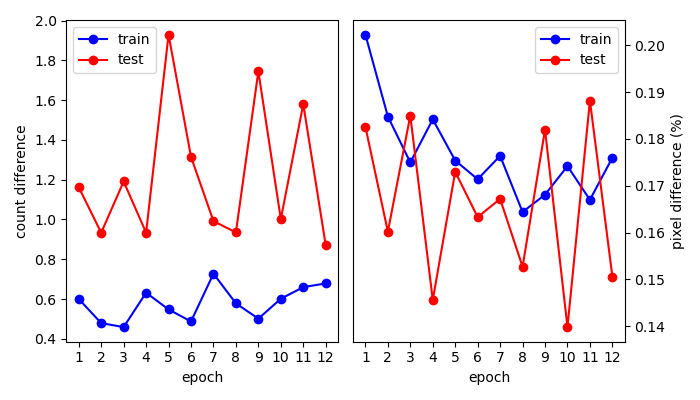
\includegraphics[width=0.9\textwidth]{epoch_summary_to_epoch12.png}
  \captionsetup{width=0.9\textwidth}
  \caption{Although the training dataset performed well, the validation 
  dataset produced sporadic results.}
  \label{fig:epoch-summary}
\end{figure}

\section{Discussion}

By building and training a CNN with Gunpowder and PyTorch, we have 
successfully constructed an automatic microglia identification model. As 
shown in Figure \ref{fig:epoch-summary}, the pixel accuracy of our model is 
quite high, which indicates that false positives or false negatives are rare, 
and the predicted shape of the microglia are approximately as expected.

In the future, these accuracy metrics will be compared with the accuracy of a 
human annotator by having many different experts manually identify microglia 
in the same images, then compare the difference between their results. While 
there are still some false positives and negatives, the model trains 
incredibly quickly, as can be seen in Table \ref{tbl:epoch-summary} by how 
good the initial results are in the first epoch of training. 

Using the guidance of other similar models, we were able to construct an 
accurate model without much parameter tweaking. Unfortunately, due to time 
constraints and the extensive training time required, we were unable to 
conduct large hyperparameter tuning experiments to improve our model results. 
However, these experiments will be done in the wake of this course project 
before handing off the model to the Tremblay Lab for research use. It is 
expected that through modifying the parameters of the model, the results will 
continue to improve.

The results in Table \ref{tbl:epoch-summary} seem to indicate that our model 
is overfitting when it comes to our count difference metric, since the 
training set accuracy is consistently better than the test set accuracy. 
However, the pixel difference metric indicates that the test set accuracy is 
better than the training set. While the accuracy difference isn't huge, this 
is an unexpected result and is worth investigating further. It may be that 
the model has difficulty predicting microglia along the edge of an image, 
which would mean that the pixel difference accuracy on a larger image will be 
better since the ratio between the image area and the image perimeter 
increases as the image size increases. Since the test set images are larger 
(500x500) than the training set images (200x200), this might explain the 
unexpected difference in pixel difference accuracy.

Table \ref{tbl:img-summary} illustrates the varied performance across the 
different images, and indicates a pattern of exponential increase in the 
predictions as the actual number of microglia increases. This may account for 
the correspondingly higher error associated with these images, and provides 
opportunity to investigate why this is happening.

In the process of preparing the brain sample for light microscopy, the tissue 
sample is stained to highlight the target cells. It was observed that the 
degree of staining and image focus varied between source images, and may have 
contributed to some variability in the predictions, as the model likely made 
predictions largely on the spatial distribution of colour. As the model 
matures and becomes used by the Lab as a tool in their process, it may 
improve at handling these staining and focusing imperfections. The Lab is 
also working to improve their tissue staining and image focusing quality, so 
our model accuracy is likely to improve as their data quality increases.

In the coming weeks, this model will be tested on larger images to simulate 
how the Lab will use it, and hyperparameter experiments will be conducted to 
decrease the error even further. Once the Lab is satisfied with the model's 
accuracy, the project will shift to using the new morphology dataset to begin 
training the morphology CNN. Since our method of identifying microglia 
involves segmenting the cell body, we hope that the same model parameters 
will produce good results for the morphology CNN with only minimal tweaking. 
The Tremblay Lab has recently acquired a FIB-SEM, which will produce 
incredibly high precision 3D electron microscopy images, and our work on this 
project will be adapted to do the 3D analysis on these higher precision image 
stacks.

\FloatBarrier

\newpage
\section{References}

\printbibliography[heading=none]

\end{document}
